\documentclass[aspectratio=169,10pt]{beamer}
\usepackage{teaching_slides}


\title{The non-parametric/machine learning future?}
\author{Chris Conlon}
\institute{NYU Stern}
\date{Fall 2026}


% for matrix decomp
\usepackage{stackengine}
\stackMath
\newlength\matfield
\newlength\tmplength
\def\matscale{1.}
\newcommand\dimbox[3]{%
  \setlength\matfield{\matscale\baselineskip}%
  \setbox0=\hbox{\vphantom{X}\smash{#3}}%
  \setlength{\tmplength}{#1\matfield-\ht0-\dp0}%
  \fboxrule=1pt\fboxsep=-\fboxrule\relax%
  \fbox{\makebox[#2\matfield]{\addstackgap[.5\tmplength]{\box0}}}%
}
\newcommand\raiserows[2]{%
   \setlength\matfield{\matscale\baselineskip}%
   \raisebox{#1\matfield}{#2}%
}
\newcommand\matbox[5]{
  \stackunder{\dimbox{#1}{#2}{$\mathbf{#5}$}}{\scriptstyle(#3\times #4)}%
}


\begin{document}



%--------------
% TITLE PAGE
\begin{frame}
\titlepage
\end{frame}


\section*{Nonparametrics?}


\begin{frame}{What do you mean by non-parametric?}
Mostly we mean putting a flexible distribution on $f(\beta_i,\alpha_i \mid \theta)$ (and keeping logit error on $\varepsilon_{ij}$)
\begin{align*}
u_{ij} = \beta_i x_j - \alpha_i p_j + \xi_j + \varepsilon_{ij} \text{ with } f(\beta_i,\alpha_i \mid \theta)
\end{align*}
\begin{itemize}
    \item Fixed Grids (Fox, Kim, Ryan, Bajari 2011, Heiss, Hetzenecker, Osterhaus 2022, Nevo Turner Williams 2016): draw from ``prior'' of $\beta_i$, compute $\sigma_{ij}(\beta_i)$ and choose weights on each $i$, $\pi_i$.
    \item Compiani (QE 2022): approximate $\sigma_{j}^{-1}(\calS_t,\symbf{x}_t^{(2)})$ directly with Bernstein Polynomials (ditches $\varepsilon \rightarrow$ very hard)
    \item Ao Wang (JE 2022): use polynomial sieves: $\mathbb{E}\left[\left(\sigma_j^{-1}\left(\calS_t ; \symbf{x}_t^{(2)}, \alert{F}\right)-X_t^{(1)} \beta^{(1)}\right) \phi_k\left(Z_{j t}\right)\right]=0$
    \item Lu, Shi, Tao (JE 2023): use partially linear model: $\log \left(s_{j t} / s_{0 t}\right)=X_{1, j t}^{\prime} \beta^0+\alert{\psi^0\left(X_{2, j t} ; IV_{J, t}\right)}+\xi_{j t}$ where        $\psi^0\left(x_{2, j t} ; IV_{J, t}\right)=\log \left[\frac{\int \frac{\exp \left(x_{2, j t}^{\prime} v\right)}{\exp \left(IV_{J, t}(v)\right)} f^0(v) d v}{\int \frac{1}{\exp \left(IV_{J, t}(v)\right)} f^0(v) d v}\right]$.
\end{itemize}
But these are still \alert{only as good as characteristics}.
\end{frame}

\begin{frame}{Idea \#1: t-STE Embeddings (Van Der Maaten and Weinberger, 2012)}
\begin{itemize}
  \item \textbf{Goal:} Assign a low-dimensional vector of characteristics $x_{j} \in \mathbb{R}^m$ for each product using triplets of the form
  “$j$ is more similar to $k$ than to $\ell$”.
  \vspace{0.6em}
  \item The “t” in t-STE comes from using a \textbf{Student-t kernel} 
  to model distances—giving heavy tails and better separation of clusters.
  \begin{align*}
\max _{\mathbf{x}} \sum_{(j, k,\ell) \in \mathcal{T}} \ln \left(\pi_{j k \ell}\right) \quad \text { where } \quad \pi_{ j k \ell}=\frac{\left(1+\frac{\left\|x_j-x_{\ell}\right\|^2}{\alpha}\right)^{-\frac{\alpha+1}{2}}}{\left(1+\frac{\left\|x_j-x_k\right\|^2}{\alpha}\right)^{-\frac{\alpha+1}{2}}+\left(1+\frac{\left\|x_j-x_{\ell}\right\|^2}{\alpha}\right)^{-\frac{\alpha+1}{2}}}
  \end{align*}
  \item This is basically maximium (log) likelihood for a binary outcome model (closer to $\ell$ than $k$).
  \begin{itemize}
        \item Fit with canned routine (which does gradient descent).
        \item $\alpha$ is a (somewhat arbitrary) tuning parameter.
   \end{itemize}

\end{itemize}
\end{frame}




\begin{frame}{Unobserved Characteristics: Magnolfi Maclure Sorensen (2023)}
\begin{columns}
\begin{column}{0.5\textwidth}
     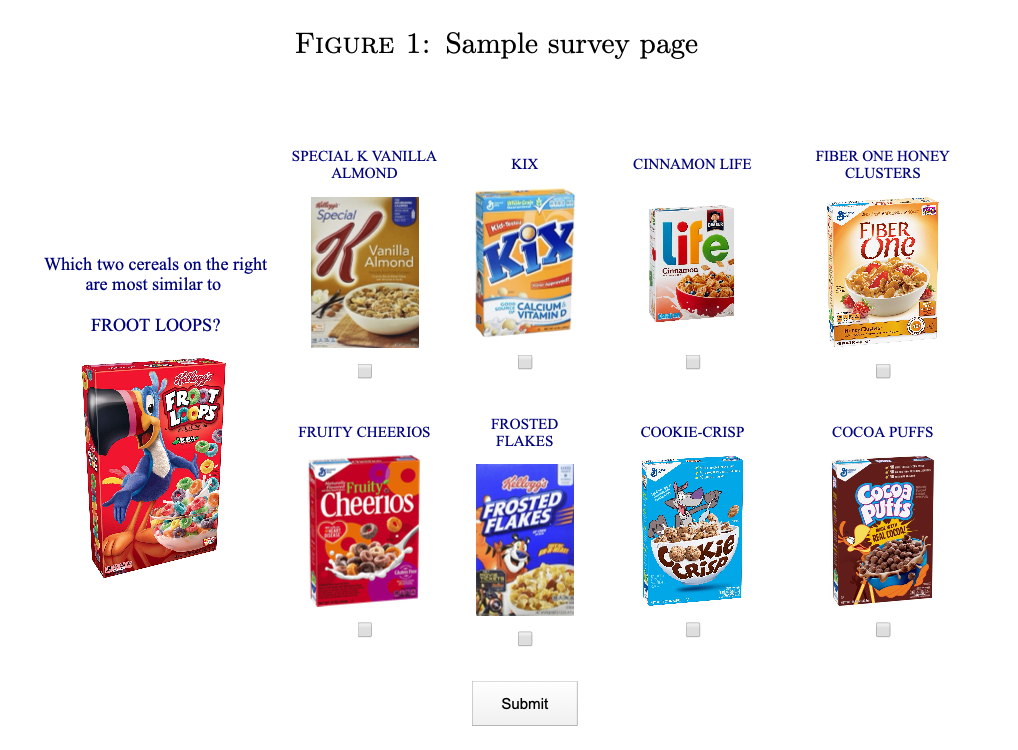
\includegraphics[width=\textwidth]{resources/embeddings_1}      
\end{column}
\begin{column}{0.5\textwidth}
What if we could first estimate \alert{unobserved characteristics}?
\begin{itemize}
\item Is $j$ more similar to $k$ or $l$?
\item Get a $m \times J$ matrix with $m$ factors (embeddings).
\item Idea: $m$ is small (like 3-4).
\item Use these as characteristics in BLP demand model.
\end{itemize}
\end{column}
\end{columns}
\end{frame}


\begin{frame}{Unobserved Characteristics: Magnolfi McClure Sorensen (2023)}
\begin{columns}
\begin{column}{0.5\textwidth}
     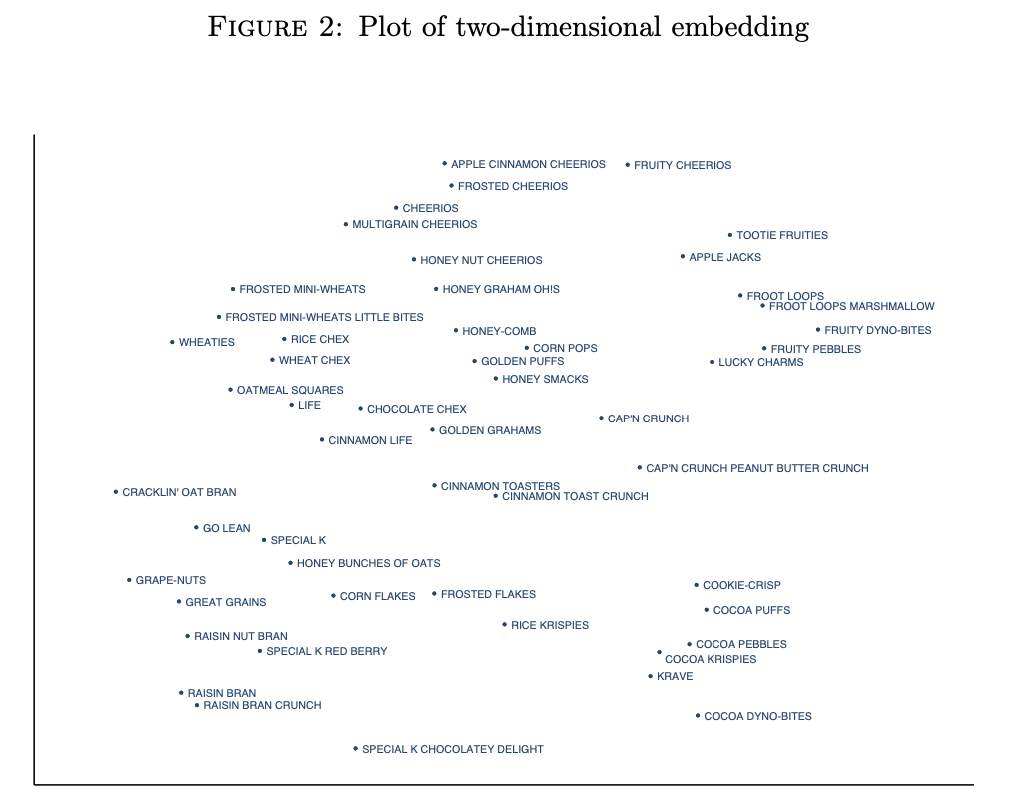
\includegraphics[width=\textwidth]{resources/embeddings_2}      
\end{column}
\begin{column}{0.5\textwidth}
     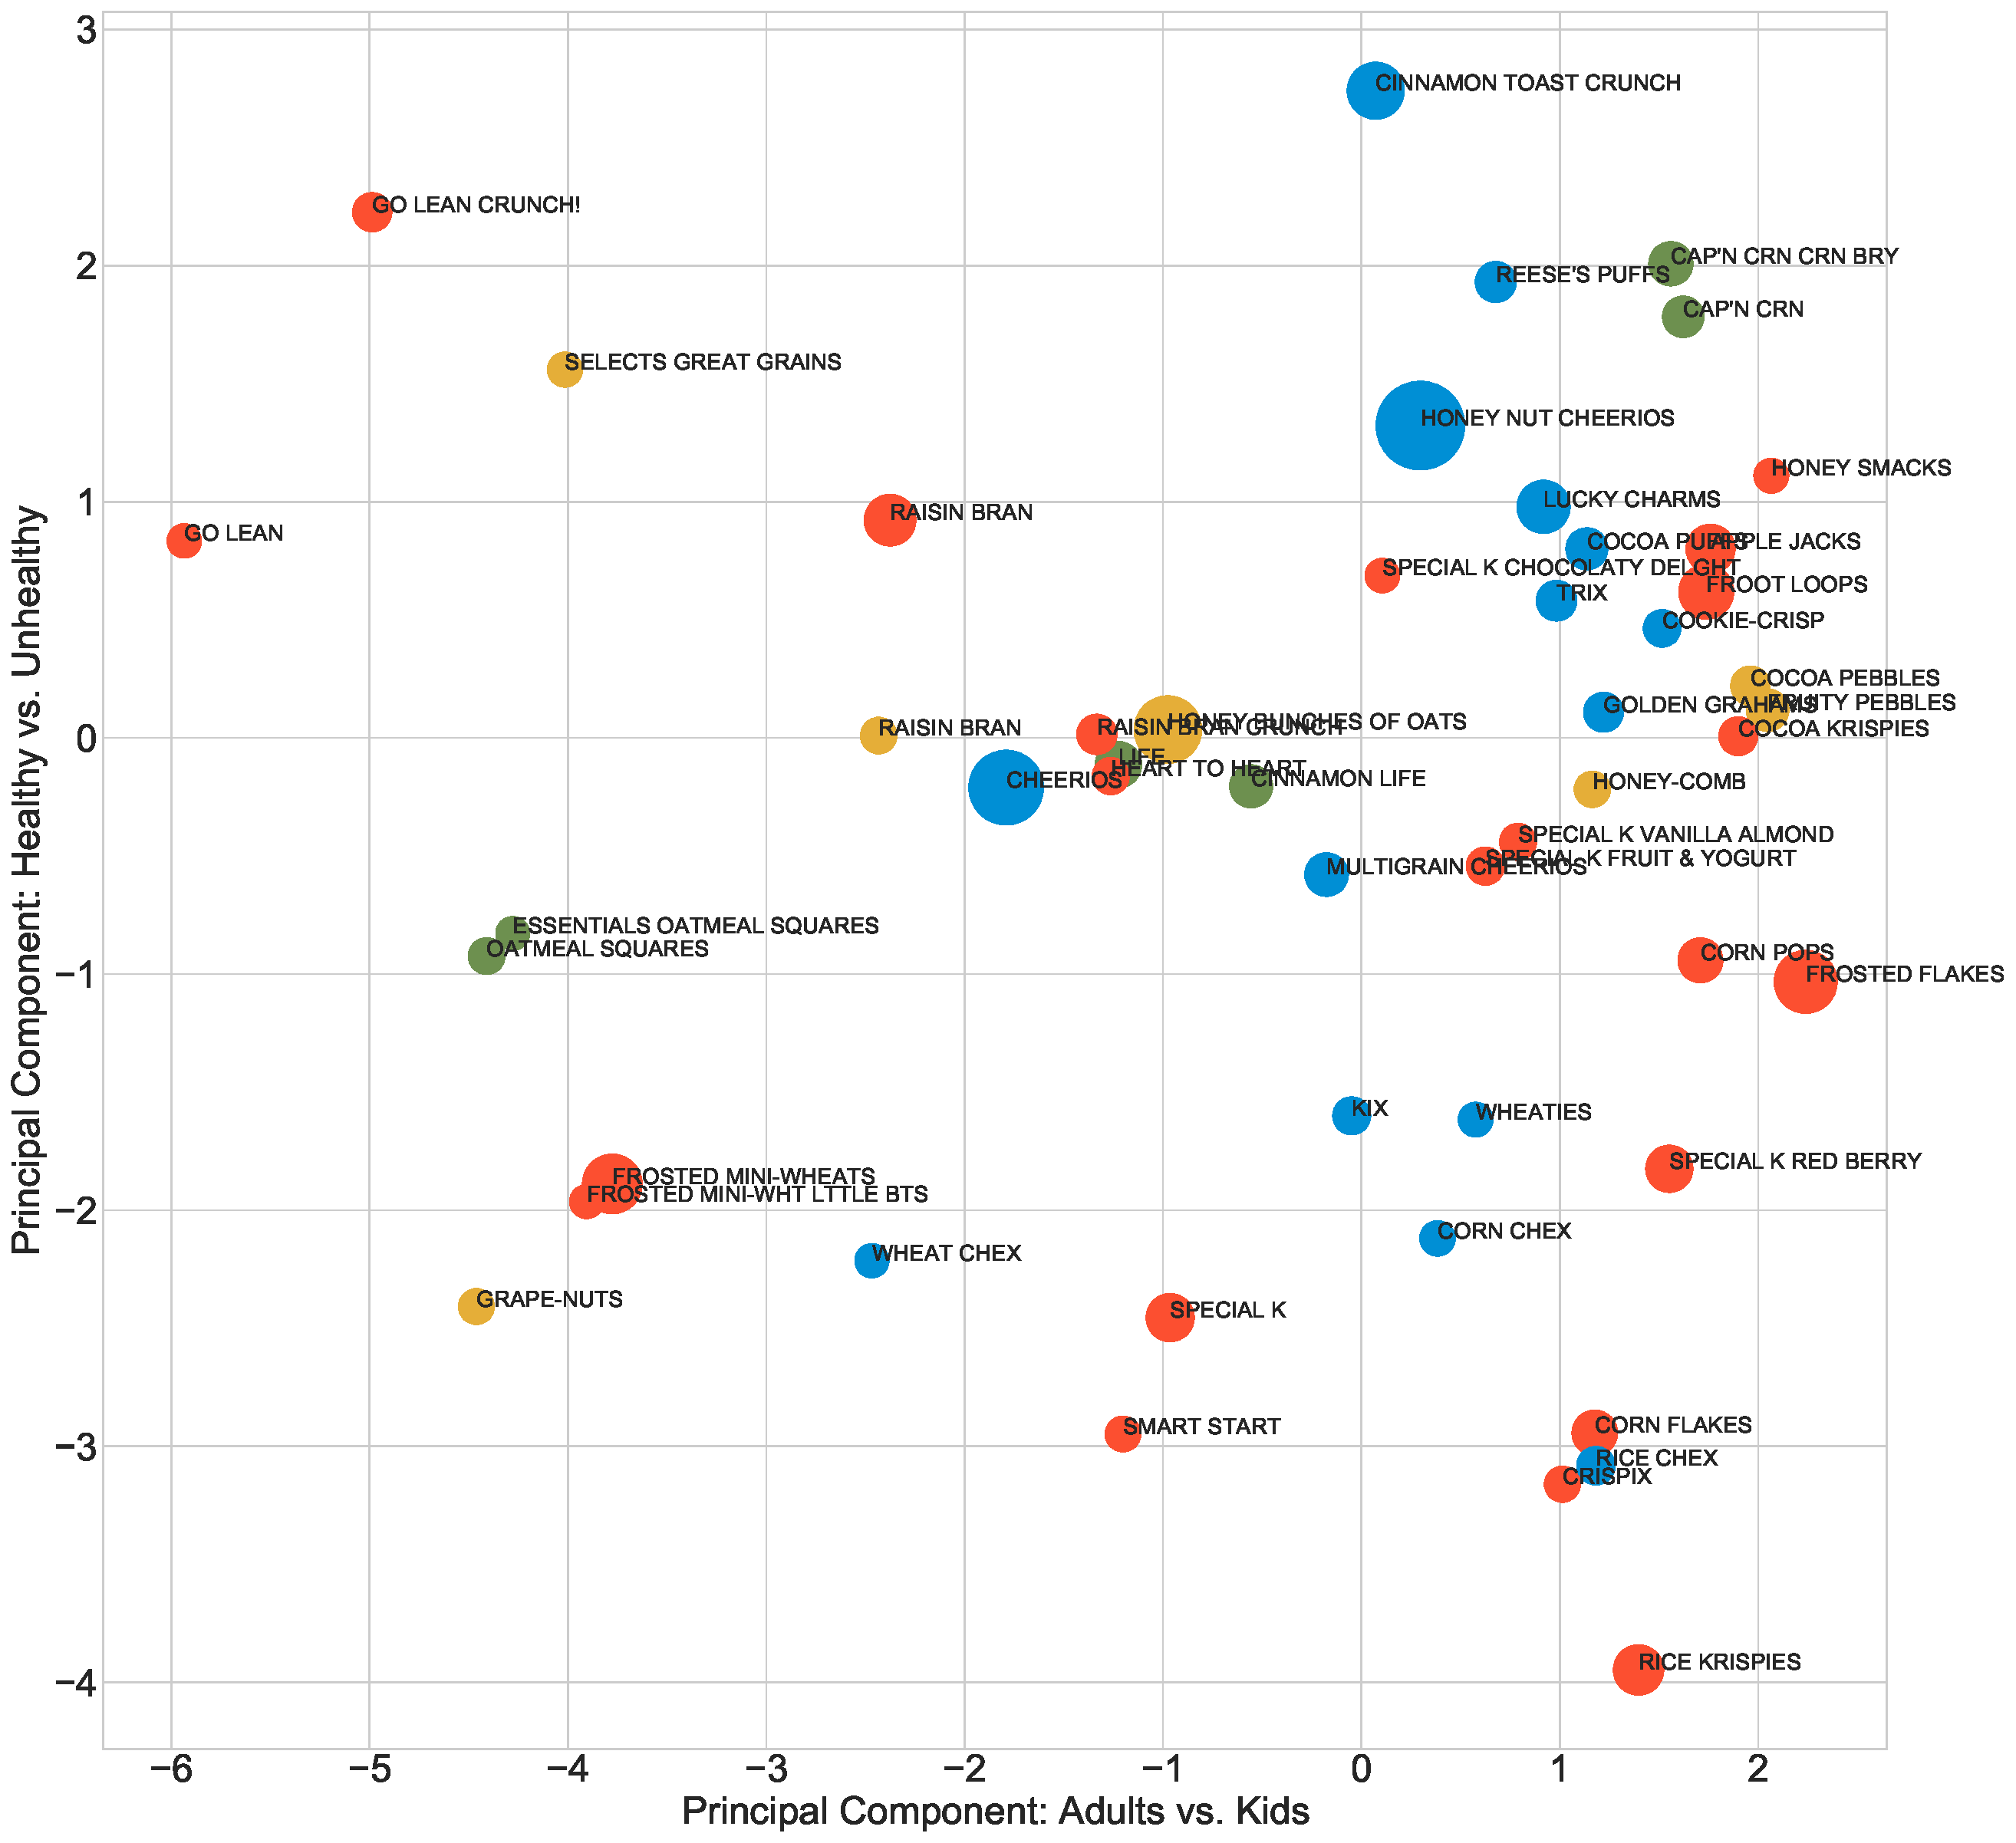
\includegraphics[width=\textwidth]{resources/pca_01}
\end{column}
\end{columns}
\end{frame}

\begin{frame}{Reverse Engineering Hotel Recommendations:  McClure (2025)}
\begin{columns}
\begin{column}{0.6\textwidth}
     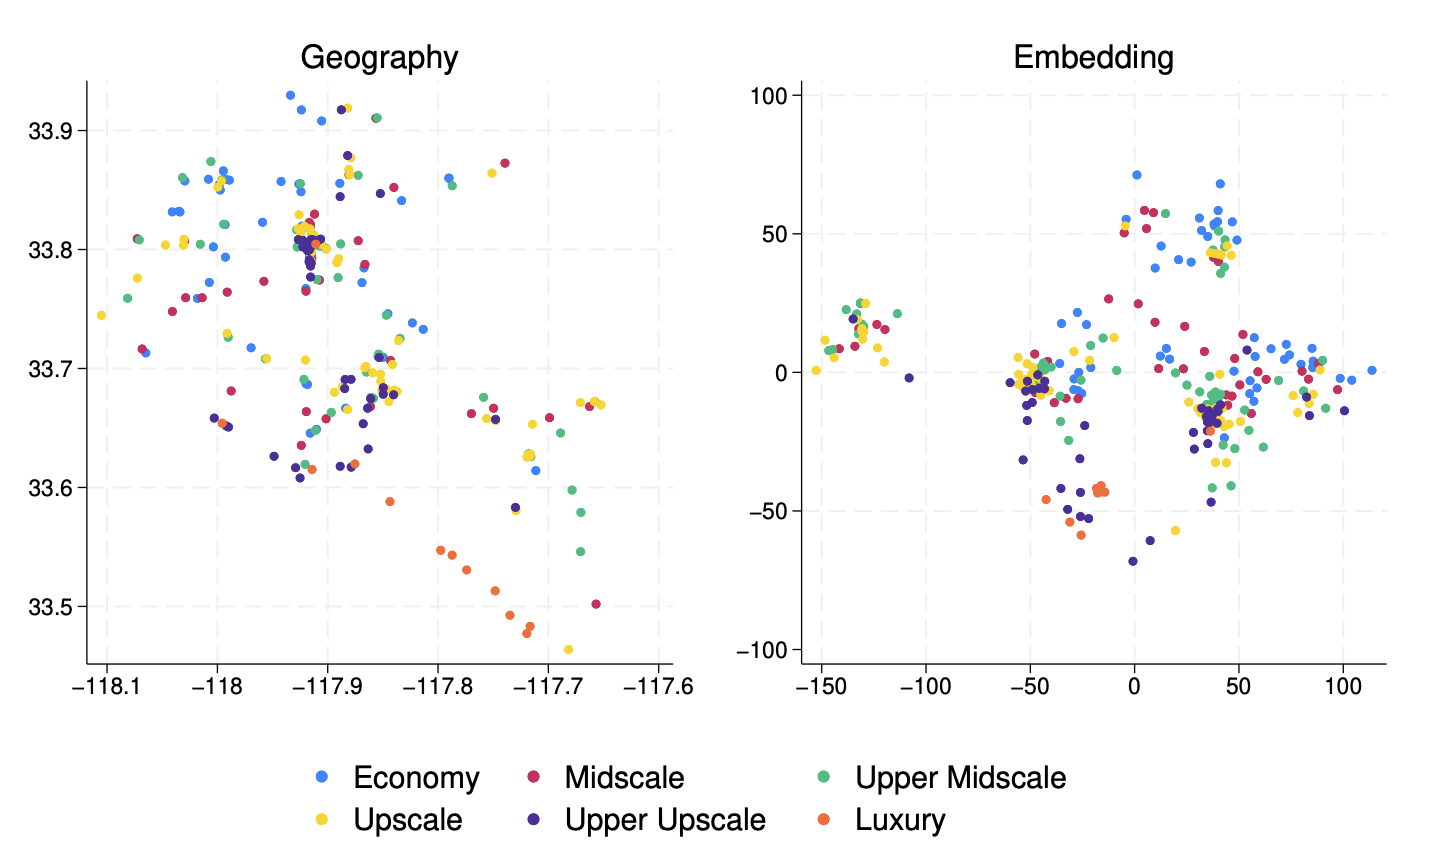
\includegraphics[height=0.5\textheight]{resources/hotel_embedding}\\
     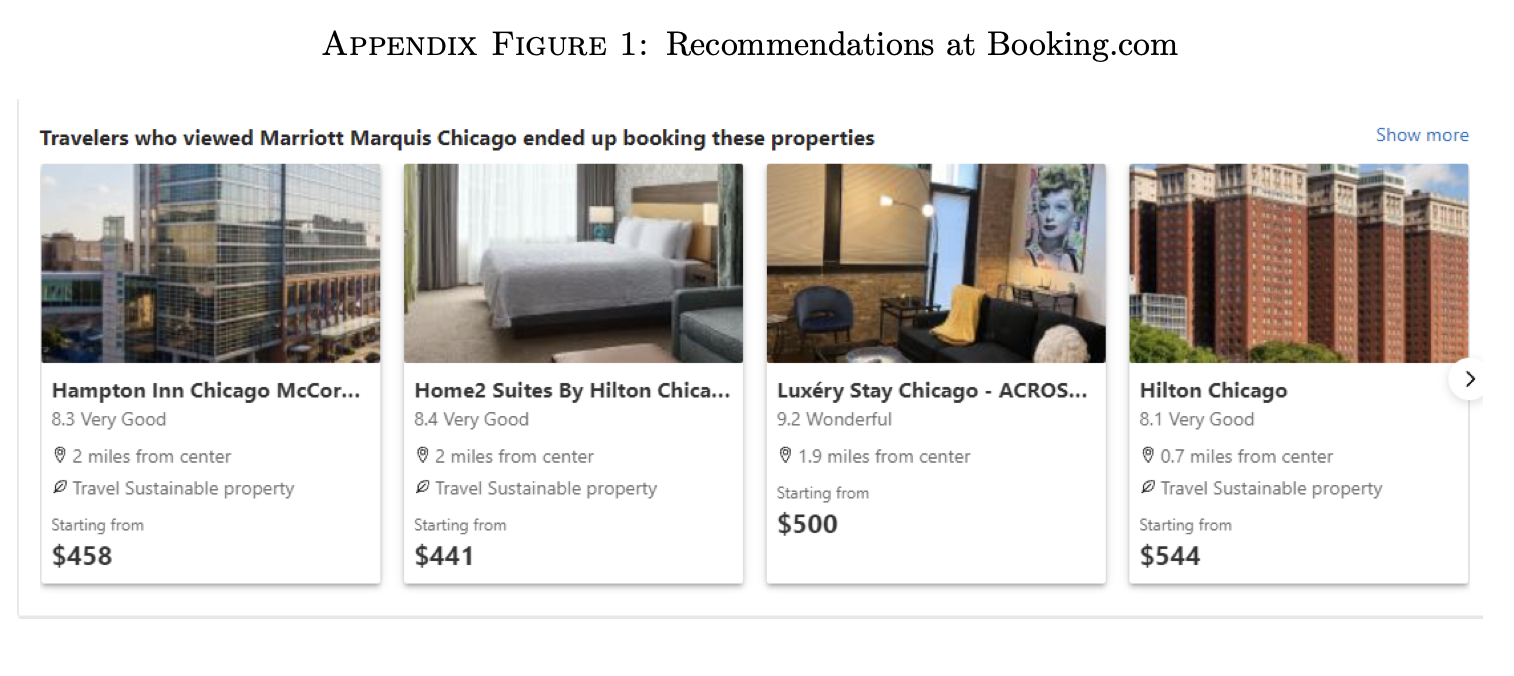
\includegraphics[height=0.5\textheight]{resources/hotel_ranking}
\end{column}
\begin{column}{0.4\textwidth}
    \begin{itemize}
        \item Scrape observed ``you may also like'' recommendations from hotels and use those to construct \alert{triplets}
        \item Feed the triplets into tSTE embedding model to get a matrix $\mathbf{X}$: ($J \times F$) where $F$ is small (2-3).
        \item In both cases plug these in as characteristics to demand model (no guarantee they explain substitution patterns).
    \end{itemize}
\end{column}
\end{columns}

\end{frame}




\begin{frame}{Idea \#2: Low Rank Matrix Factorization: aka Netflix Prize}
%\renewcommand\matscale{.6}
\begin{align*}
\matbox{7}{7}{I}{J}{Ratings} = 
\matbox{7}{5}{I}{F}{Individuals} \raiserows{2.5}{\matbox{2}{7}{F}{J}{Movies}}
\end{align*}
\begin{wideitemize}
    \item Even if Ratings are \alert{sparse}, we fit the observed cells and predict the rest!
    \item Idea: Approximate with a low rank $(F)$ factor model (such as SVD)
    \item Maybe embeddings are reverse-engineering ``collaborative filter''.
    \end{wideitemize}
\end{frame}



\begin{frame}{Conlon, Mortimer, Sarkis (2024): Structural Low Rank Approximations}
\small
Fix $\textrm{rank}(\symbf{D}(\symbf{S},\pi))=I$, and for each choice of $I$ solve:
\begin{align*}
\min _{(\symbf{S}, \pi) \geq 0} \left\|\mathcal{P}_{\Omega}(\calD-\symbf{D}(\symbf{S},\pi))\right\|_{\ell_2}  &+ \lambda \left\|\calS- \symbf{S}\,\pi \right\|_{\ell_2} \text { with } \left\|\pi  \right\|_{\ell_1} \leq 1, \quad   \left\|\symbf{s_i}  \right\|_{\ell_1} \leq 1.
\end{align*}
\vspace{-.25cm}
\begin{itemize}
\item Goal: estimate $\symbf{s_i}$ (choice probabilities) and corresponding weights $\pi_i$ (Finite Mixture) in \alert{product space}
\begin{itemize}
\item Consistent with $U_{ij} = V_{ij} + \varepsilon_{ij}$ and logit error.
\end{itemize}
\item Constraints: Choice probabilities $s_{ij}$ sum to one, type weights $\pi_i$ sum to one.
\begin{itemize}
\item $\ell_1$ constraints lead to \alert{sparsity}.
\end{itemize}
\item Idea: \alert{Control the rank by limiting $I$ directly}
\begin{itemize}
\item Use cross validation to select \# of types $I$ and Lagrange multiplier $\lambda$.
\end{itemize}
\item Matrix completion: We can construct estimates of $\symbf{D}(\symbf{S},\pi)$ including elements of $\mathcal{P}_{\overline{\Omega}}$.
\begin{align*}
%    & s_j = \sum_{i} \pi_i s_{i,j} \text{ for all } j \in \mathcal{J}\\
    & \symbf{D}= \frac{1}{\symbf{s}}\sum_{i = 1}^I \pi_i \, \symbf{s_i} \times \left[\frac{\symbf{s_{i}}}{1-\symbf{s_i}}\right]^T
\end{align*}
% \item Weights $\widetilde c_j$ and $c_j$ are proportional to $\ln q_j$
\end{itemize}
\end{frame}


\begin{frame}{Profiles of Types (Rank 15)}
\begin{columns}
\begin{column}{0.5\textwidth}
    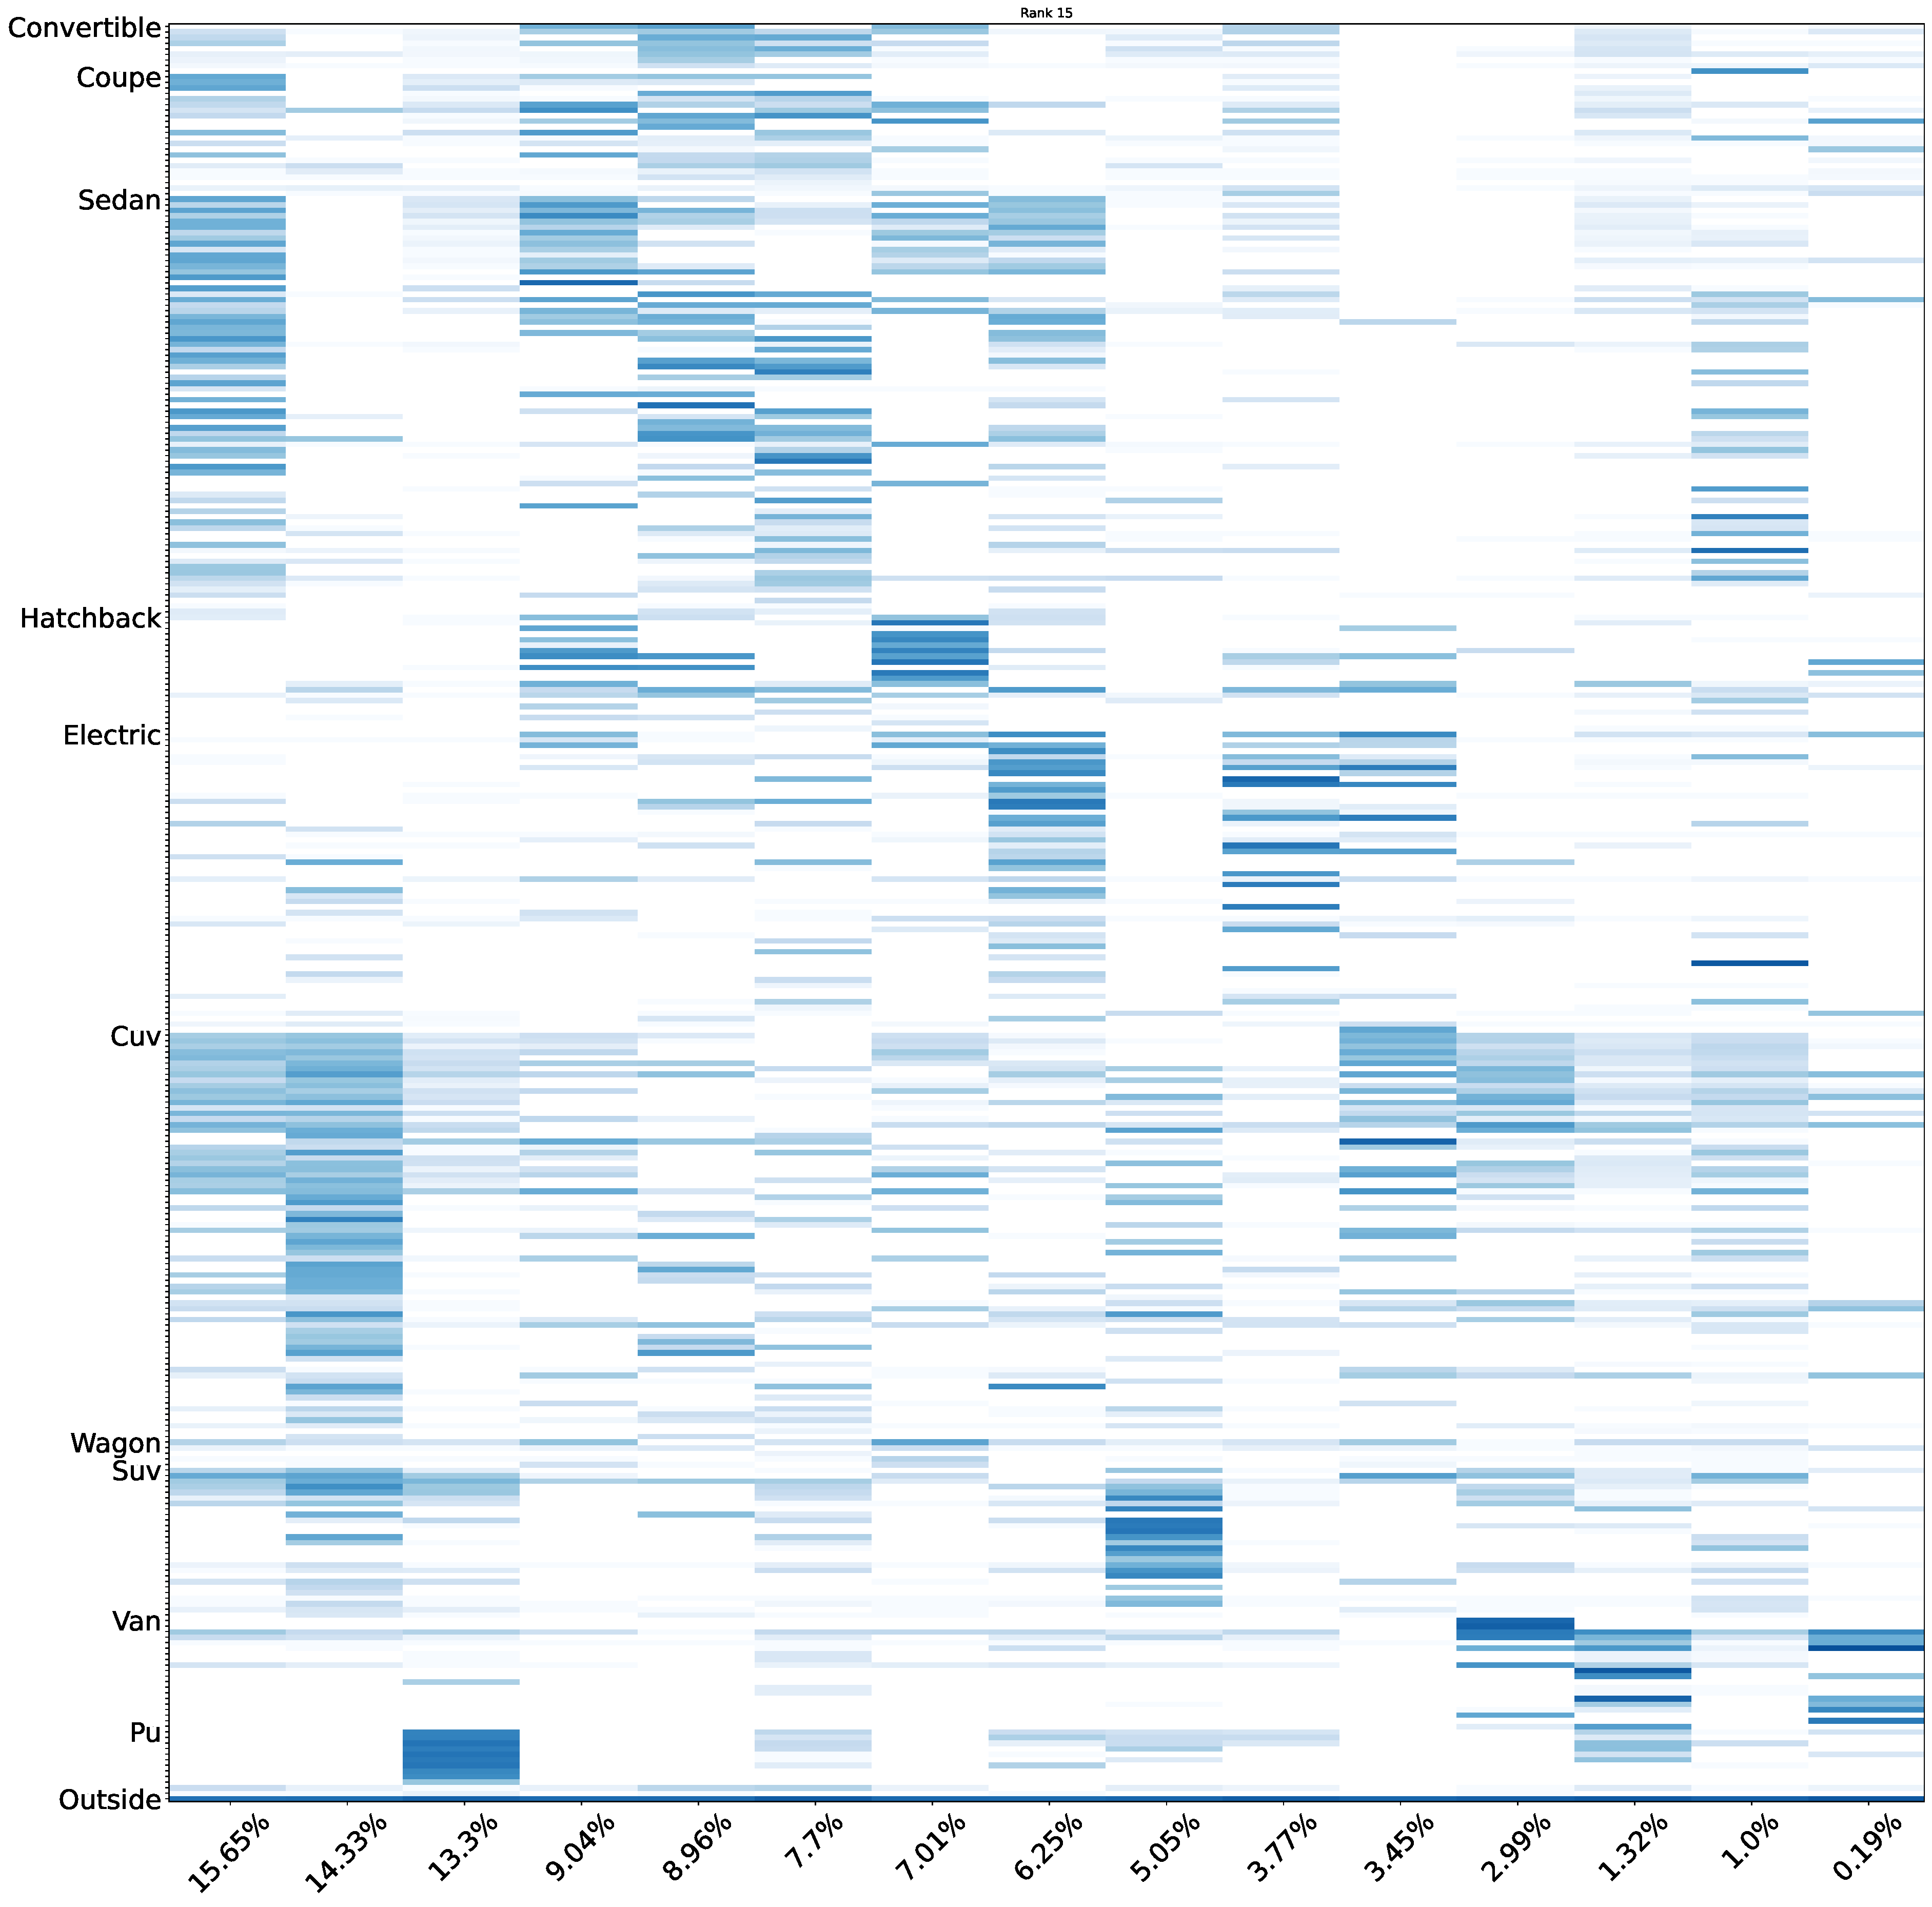
\includegraphics[height=0.95\textheight]{resources/hpc_rank_15_profiles}
\end{column}
\begin{column}{0.5\textwidth}
    \begin{itemize}
        \item Each column of the matrix $\symbf{S}$ ($I \times J$) represents a ``type'' $\symbf{s_i}$ (a $J \times 1$) vector of choice probabilities.
        \item We see both the \alert{sparsity} as well as specific consumer \alert{segments} (or ``types'').
        \item We also obtain the share of each type in the population $\pi_i$.
        \item Remember that $u_{ij} - u_{i0} = \log s_{ij} - \log s_{i0}$, so that we identify indirect utilities (relative to outside good).
        \item We still need to estimate $\frac{\partial u_{ij}}{\partial p_j}$ somehow.
    \end{itemize}
\end{column}
\end{columns}
\end{frame}


\begin{frame}{In-Sample Performance}
\label{in_sample}
%\hyperlink{cross_valid}{\beamerbutton{Cross Validation}}
\centering
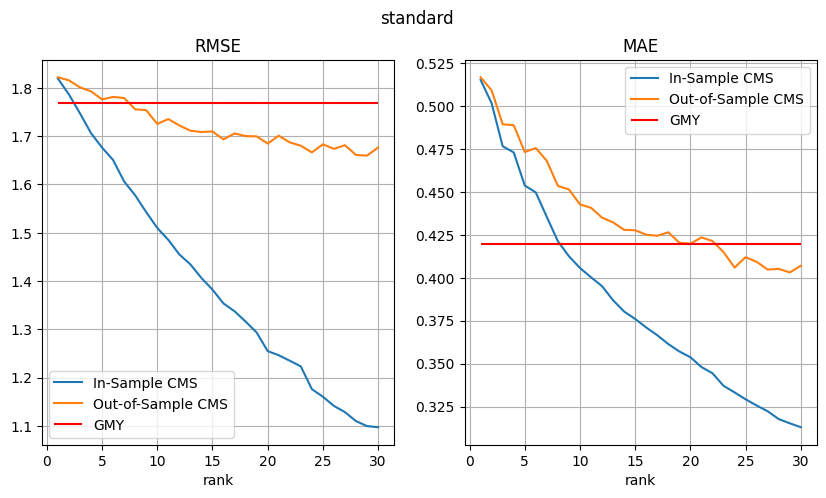
\includegraphics[height=\textheight,width=\textwidth, keepaspectratio]{resources/standard_lambda_tuned.png}\\
\end{frame}




 \begin{frame}{Top Substitutes: Ford F-Series}
    \centering
    \begin{tabular}{rrrrrr}
  \hline
  \textbf{Model} & \textbf{Raw} & \textbf{Logit} & \textbf{CMS I=15} & \textbf{CMS I=30} & \textbf{GMY} \\\hline
  Ram Pickup & 24.59 & 0.88 & 21.46 & 22.23 & 19.4 \\
  Gmc Sierra & 20.29 & 0.61 & 14.97 & 21.92 & 17.27 \\
  Chevrolet Silverado & 15.62 & 0.78 & 13.408 & 19.63 & 33.62 \\
  Toyota Tundra & 12.98 & 0.55 & 16.32 & 12.79 & 2.29 \\
  Toyota Tacoma & 6.31 & 0.76 & 3.39 & 3.13 & 2.83 \\
  Chevrolet Colorado & 4.64 & 0.63 & 3.22 & 2.86 & 2.87 \\
  Gmc Canyon & 2.3 & 0.3 & 0.76 & 1.38 & 1.02 \\
  Nissan Frontier & 1.63 & 0.43 & 0.92 & 1.69 & 0.61 \\
  Jeep Wrangler & 1.59 & 0.69 & 1.33 & 0.94 & 0.06 \\
  Nissan Titan & 0.7 & 0.05 & 1.18 & 1.17 & 0.18 \\
  Ford Explorer & 0.63 & 0.38 & 0.16 & 0.14 & 0.71 \\\hline
\end{tabular}
\\
 \end{frame}





\begin{frame}{Idea \#3: Customer Overlap (Einav, Guido, Klenow 2025)}
\begin{columns}
\begin{column}{0.5\textwidth}
     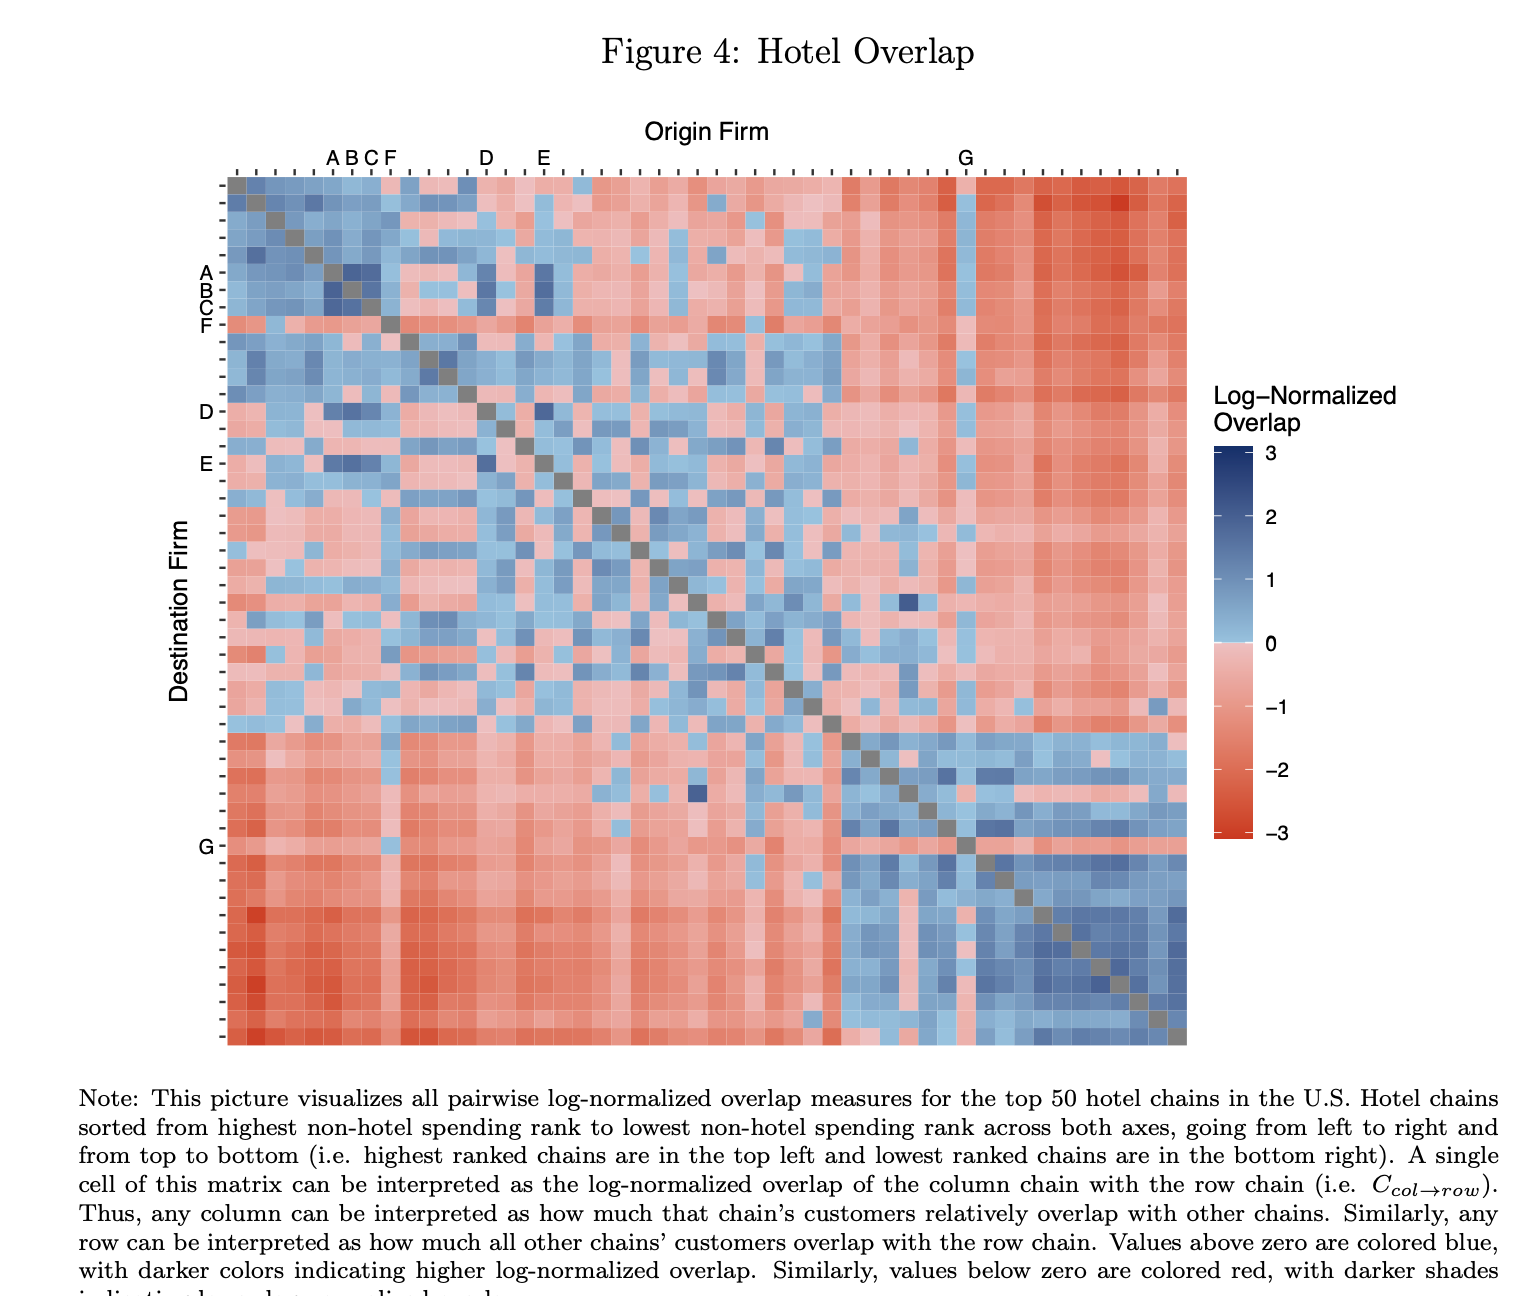
\includegraphics[width=\textwidth]{resources/einav_overlap}      
\end{column}
\begin{column}{0.5\textwidth}
    \begin{itemize}
        \item Encode a $J \times 1$ vector $\symbf{q_i}$ of every purchase (0/1) within the category for the year
        \item They use credit card data (don't see items, only stores).
        \item Could use Nielsen panelists.
        \item How many customers do two stores have in common? $C_{j \rightarrow k}=\frac{\sum_{i \in \mathcal{C}_j} q_{i,k}}{\sum_{i \in \mathcal{C}_j} q_{i,(-j)}}$.
        \item Use to estimate diversion ratios (but not a demand model). 
        \item Conlon Rao (JPE, forthcoming) use a similar measure to estimate nesting parameter.
        \item Atalay et. al (JPE, 2024) use a similar measure to assign products to nests.
    \end{itemize}
\end{column}
\end{columns}
\end{frame}

\section{Thanks!}


\end{document}